\documentclass[a4paper,12pt]{report}

\usepackage[utf8x]{inputenc}
\usepackage[T2A]{fontenc}
\usepackage[english, russian]{babel}
\usepackage[table]{xcolor}

% Опционно, требует  apt-get install scalable-cyrfonts.*
% и удаления одной строчки в cyrtimes.sty
% Сточку не удалять!
% \usepackage{cyrtimes}

% Картнки и tikz
\usepackage{graphicx}
\usepackage{tikz}
\usetikzlibrary{snakes,arrows,shapes}


% Увы, поля придётся уменьшить из-за листингов.
\topmargin -1cm
\oddsidemargin -0.5cm
\evensidemargin -0.5cm
\textwidth 17cm
\textheight 24cm

\sloppy

% Оглавление в PDF
\usepackage[
bookmarks=true,
colorlinks=true, linkcolor=black, anchorcolor=black, citecolor=black, menucolor=black,filecolor=black, urlcolor=black,
unicode=true
]{hyperref}

% Для исходного кода в тексте
% \newcommand{\Code}[1]{\texttt{#1}}

% Некоторая русификация.
% \usepackage{misccorr} % Oh shi^W^W, оно не работает с report.
\usepackage{indentfirst}
\renewcommand{\labelitemi}{\normalfont\bfseries{--}}

% На дворе XXI век, но пакет listings всё ещё не пашет с русскими комментариями!

% Пакет listings для простой вставки исходников
% \usepackage{listings}
% Параметры оформления
% \lstset{
% showspaces=false,
% showtabs=false,
% frame=single,
% tabsize=4,
% basicstyle=\ttfamily,
% identifierstyle=\ttfamily,
% commentstyle=\itshape,
% stringstyle=\ttfamily,
% keywordstyle=\ttfamily,
% breaklines=true
% }
% Русский в комментариях.
% \lstset{escapebegin=\begin{cyr},escapeend=\end{cyr}}

% От доксиджена
\usepackage{ifthen}
\ifx\requestedLaTeXdate\undefined
\usepackage{array}
\else
\usepackage{array}[=2016-10-06]
\fi
%%
% Packages required by doxygen
\usepackage{fixltx2e}
\usepackage{calc}
\usepackage{doxygen}
\usepackage{graphicx}
\usepackage{makeidx}
\usepackage{multicol}
\usepackage{multirow}
\PassOptionsToPackage{warn}{textcomp}
\usepackage{textcomp}
\usepackage[nointegrals]{wasysym}
\usepackage{ifpdf,ifxetex}

% NLS support packages
\usepackage[T2A]{fontenc}
\usepackage[russian]{babel}

% Font selection
\usepackage[T1]{fontenc}
\usepackage[scaled=.90]{helvet}
\usepackage{courier}
\usepackage{amssymb}
\usepackage{sectsty}

\newcommand{\+}{\discretionary{\mbox{\scriptsize$\hookleftarrow$}}{}{}}

% Arguments of doxygenemoji:
% 1) ':<text>:' form of the emoji, already "LaTeX"-escaped
% 2) file with the name of the emoji without the .png extension
% in case image exist use this otherwise use the ':<text>:' form
\newcommand{\doxygenemoji}[2]{%
  \IfFileExists{./#2.png}{\raisebox{-0.1em}{\includegraphics[height=0.9em]{./#2.png}}}{#1}%
}
% Page & text layout
\usepackage{geometry}
\geometry{%
  a4paper,%
  top=2.5cm,%
  bottom=2.5cm,%
  left=2.5cm,%
  right=2.5cm%
}
\tolerance=750
\hfuzz=15pt
\hbadness=750
\setlength{\emergencystretch}{15pt}
\setlength{\parindent}{0cm}
\newcommand{\doxynormalparskip}{\setlength{\parskip}{3ex plus 2ex minus 2ex}}
\newcommand{\doxytocparskip}{\setlength{\parskip}{1ex plus 0ex minus 0ex}}
\doxynormalparskip


\makeatletter
\newcommand\hrulefilll{\leavevmode\leaders\hrule\hskip 0pt plus 1filll\kern\z@}
\makeatother

% Headers & footers
\usepackage{fancyhdr}

% Indices & bibliography
\usepackage{natbib}
\usepackage[titles]{tocloft}
\setcounter{tocdepth}{3}
\setcounter{secnumdepth}{5}
\makeindex

\usepackage{newunicodechar}
  \newunicodechar{⁻}{${}^{-}$}% Superscript minus
  \newunicodechar{²}{${}^{2}$}% Superscript two
  \newunicodechar{³}{${}^{3}$}% Superscript three

% Custom commands
\newcommand{\clearemptydoublepage}{%
  \newpage{\pagestyle{empty}\cleardoublepage}%
}

\usepackage{caption}
\captionsetup{labelsep=space,justification=centering,singlelinecheck=off,skip=4pt,position=top}

\usepackage{etoc}
\etocsettocstyle{\doxytocparskip}{\doxynormalparskip}
\renewcommand{\numberline}[1]{#1~}




\title{Расчетно-Пояснительная Записка \\ 
    \large к курсовой работе на тему: \\ Клиентская часть MTA SMTP}
\author{ИУ7-33М Зыкин Д.А.}

\begin{document}

\maketitle


\tableofcontents

\clearpage
\chapter*{Введение}
\addcontentsline{toc}{chapter}{Введение}

Данная расчетно-пояснительная записка содержит информацию о протоколе SMTP (англ. \textbf{S}imple \textbf{M}ail \textbf{T}ransfer \textbf{P}rotocol) и реализации серверной части MTA (англ. \textbf{M}essage \textbf{T}ransfer \textbf{A}gent) SMTP в рамках курсовой работы.

Задание: необходимо было создать SMTP-клиент, как часть MTA, обеспечивающий удаленную доставку и поддерживающий очереди сообщений. Дополнительные условия:
\begin{itemize}
\item Используется системный вызов \texttt{select()};
\item Используется несколько рабочий процессов;
\item Журналирование в отдельном процессе.
\end{itemize}

Цель работы: реализовать клиентскую часть MTA SMTP.

Основные задачи:
\begin{enumerate}
    \item Анализ и изучение протокола SMTP, способов мультиплексирования;
    \item Программная реализация SMTP клиента на языке программирования Си под Unix-подобные операционные системы;
    \item Тестирование и отладка написанного клиента;
    \item Оформление расчетно-пояснительной записки по результатам работы.
\end{enumerate}


\chapter{Аналитический раздел}


\section{Протокол SMTP}

SMTP (англ. \textbf{S}imple \textbf{M}ail \textbf{T}ransfer \textbf{P}rotocol) ~-- это широко используемый сетевой протокол, предназначенный для передачи писем электронной почты в сетях TCP/IP. SMTP впервые был описан в RFC 821 (1982 год), а последнее обновление описано в RFC 5321 (2008 год) и включает масштабируемое расширение протокола — ESMTP (Extended SMTP). В настоящее время под протоколом SMTP подразумеваются и его расширения. Протокол SMTP предназначен для передачи исходящей почты с использованием порта TCP 25.

Взаимодействие в рамках SMTP строится по принципу двусторонней связи, которая устанавливается между отправителем и получателем почтового сообщения. При этом отправитель инициирует соединение и посылает запросы, а получатель - отвечает на эти запросы. Таким образом, отправитель выступает в роли клиента, а получатель - сервера.


\subsection{Базовые команды SMTP}

Каждая команда SMTP начинается с ключевого слова – названия команды, указывающего какую операцию хочет произвести клиент. За ним могут следовать параметры, отделенные пробелом. Конец строк в протоколе SMTP обозначается последовательностью символов "возврат каретки"\ (\textbackslash r) и "перевод строки"\ (\textbackslash n) - эта последовательность обозначается CRLF. Сервер начинает выполнение команды только получив от клиента строку, завершающуюся последовательностью CRLF. 

Обычный ответ SMTP сервера на команды клиента состоит из номера ответа, за которым через пробел следует дополнительный текст. Номер ответа служит индикатором состояния сервера и делится на четыре группы:
\begin{itemize}
    \item Команда выполнена успешно (код 2xx);
    \item Промежуточный положительный результат. Команда принята, но сервер ожидает от клиента дополнительные данные для завершения операции (код 3xx);
    \item Исполнение команды временно невозможно. Команда не может быть выполнена, но проблема может быть устранена (код 4xx);
    \item Исполнение команды невозможно (код 5xx).
\end{itemize}

Если ответ состоит из нескольких строк, то каждая из них начинается номером, который отделяется от сопровождающего текста не пробелом, а символом "минус"\ (-). В последней строке номер отделяется от текста пробелом. Каждая строка ответа, как и строки команд, заканчивается последовательностью CRLF.

Ниже представлен список базовых SMTP-команд:
\begin{itemize}
    \item EHLO доменное\_имя\_клиента CRLF - Открывает ESMTP сессию. В ответ на эту команду сервер сообщает, готов ли он к продолжению диалога.
    \item HELO доменное\_имя\_клиента CRLF - Открывает SMTP сессию. В RFC 2821 рекомендуется использовать команду HELO, только если программное обеспечение не поддерживает команду EHLO. Отличие этой команды только в том, что она делает невозможным использование расширений ESMTP. Передача почты возможна только после выполнения одной из двух перечисленных выше команд.
    \item MAIL FROM: <адрес\_отправителя> CRLF - Сообщает адрес отправителя письма. Для каждого письма команда MAIL должна быть выполнена только один раз. Адрес может быть оставлен пустым: <>. Команда MAIL может быть выполнена только после успешного выполнения команды EHLO или HELO.
    \item RCPT TO: <адрес\_получателя> CRLF - Сообщает адрес получателя письма. Доставка сообщения возможна, только если указан хотя бы один адрес получателя. Команда RCPT принимает в качестве аргумента только один адрес. Если нужно послать письмо большему числу адресатов, то команду RCPT следует повторять для каждого. Команда RCPT может быть выполнена только после успешного выполнения команды MAIL.
    \item DATA CRLF - Определяет начало письма. C помощью этой команды серверу передается текст сообщения, состоящий из заголовка и отделенного от него пустой строкой тела сообщения. В ответ на правильно введенную команду DATA сервер сообщает о готовности к приему или об ошибке, если прием сообщения невозможен. Передача самого сообщения заканчивается строкой, состоящей из одной точки. Эта строка не является частью сообщения и удаляется на приемной стороне. Команда DATA может быть выполнена только после успешного выполнения хотя бы одной команды RCPT.
    \item RSET CRLF - Сброс SMTP соединения. Команда RSET аннулирует все переданные до нее на сервер данные.
    \item VRFY CRLF - Проверяет наличия указанного в качестве аргумента почтового ящика.
    \item QUIT CRLF - Закрыть SMTP сессию. Командой QUIT клиент заканчивает диалог с сервером. Сервер посылает подтверждение и закрывает соединение. Получив это подтверждение, клиент тоже прекращает связь.
\end{itemize}

\section{Плюсы и минусы использования многопроцессорного подхода обработки подключений при помощи мультиплексирования и системного вызова select()}

В рамках задания необходимо реализовать клиентскую часть MTA SMTP с использованием системного вызова \texttt{select()} в нескольких рабочих процессах. К плюсам данного подхода можно отнести:
\begin{itemize}
    \item Возможность распределения нагрузки по нескольким процессам
    \item системный вызов \texttt{select()} удобен для простых задач, не требуется работать с динамической памятью, как в  \texttt{poll()}
\end{itemize}

К недостаткам данного подхода относятся:
\begin{itemize}
    \item Системный вызов \texttt{select()} не способен обрабатывать количество сокетов, большее 1024
    \item Создание отдельных процессов - дополнительные расходы и нагрузка на систему, особенно в случае создания процессов для обработки небольшого количества писем
\end{itemize}


\section{Сущности предметной области}

Для SMTP клиента можно выделить две основные сущности, которыми необходимо оперировать (обрабатывать, сохранять):
\begin{enumerate}
    \item Соединение - текущее активное соединение с информацией о подключении (статус подключения, буферы ввода-вывода, размеры буферов)
    \item Письмо - передаваемое клиентом сообщение на сервер с заголовками (отправитель, получатель, адрес получателя и т.д.) и данными (сам текст письма).
\end{enumerate}


\chapter{Конструкторский раздел}


\section{Конечный автомат состояний сервера}

На рис.~\ref{fig:fsm} изображен конечный автомат состояний клиентской части MTA SMTP. 

\begin{figure}[h]
    \centering
    \includegraphics[width=\textwidth]{include/client_def_dot.pdf}
    \caption{Конечный автомат состояний клиента}
    \label{fig:fsm}
\end{figure}

Все команды отправки письма по протоколу SMTP выполняются последовательно. В случае возникновения ошибки или разрыва соединения, текущее соединение переходит в состояние ошибки.

\section{Описание основных структур данных}

 Основные структуры данных клиента:
\begin{itemize}
    \item Mail\_files - структура с именами файлов в очереди сообщений
    \item Mail - структура самого письма со всей информацией о отправителе, получателе, адресе сервера получателя и текстом письма
    \item SMTP\_Connection - структура соединения, с буферами приема, отправки, письмом и состоянием соединения
\end{itemize}

\section{Обработка соединений в нескольких рабочих процессах}

Ниже представлен псевдокод обработки клиентом писем в нескольких процессах:

\begin{verbatim}
    Считать все имена файлов из очереди сообщений

    Разделить письма на несколько процессов
    Цикл для каждого процесса:
        Запустить процесс, запустить обработку нескольких переданных писем
        Считать письма
        Для каждого получателя создать соединение

        Цикл пока все соединения не перейдут в одно из конечных состояний:

        Ожидание срабатывания select
        Цикл по всем дескрипторам сокетов соединений:
            Если пришло сообщение в файловый дескриптор для выхода
                Выйти

            Если пришло сообщение на сокет соединения
                Обработать ответ сервера
            Если нужно отправить сообщение серверу
                Отослать сообщение серверу

        Проверка заверщения работы соединений
    
\end{verbatim}


\section{Связь основной программы и процесса журналирования}

На рис.~\ref{fig:ipc} изображена связь между основной программой и процессом журналирования с использованием очереди сообщений.

\begin{figure}[h]
    \centering
    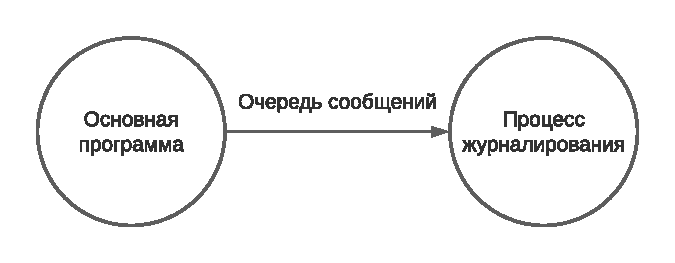
\includegraphics[width=0.7\textwidth]{pics/ipc.pdf}
    \caption{Связь основной программы и процесса журналирования}
    \label{fig:ipc}
\end{figure}


\section{Хранение почты}

Для хранения локальной почты, то есть предназначенной для клиентов с почтовым доменом сервера, используется упрощенный формат Maildir. Maildir - формат хранения электронной почты, не требующий монопольного захвата файла для обеспечения целостности почтового ящика при чтении, добавлении или изменении сообщений. Каждое сообщение хранится в отдельном файле с уникальным именем, а каждая папка представляет собой каталог. Вопросами блокировки файлов при добавлении, перемещении и удалении файлов занимается локальная файловая система. Все изменения делаются при помощи атомарных файловых операций, таким образом, монопольный захват файла ни в каком случае не нужен.

Для почты, предназначенной другим почтовым серверам также используется файловая система. Каждое сообщение аналогично хранится в отдельном файле с уникальным именем. Первоначально файл заполняется во временном месте, чтобы клиент не мог его прочитать пока тот не будет полностью записан. Затем файл переносится в отдельную заранее указанную директорию, из которой в дальнейшем клиент считывает письма для их пересылки. 

Для того, чтобы имена файлов были уникальными, в их качестве используется слегка измененный формат Unix time (рус. Unix-время) - система описания моментов во времени, принятая в Unix и других POSIX-совместимых операционных системах. В отличие от оригинального Unix time в данной работе вместо секунд, прошедших с полуночи (00:00:00 UTC) 1 января 1970 года, используются миллисекундыя, так как секунд недостаточно для удостоверения уникальности имени файла.


\chapter{Технологический раздел}


\section{Написание исходного кода}

Для написания исходного кода клиентской части MTA SMTP использовался язык C стандарта C99 со стандартными системными библиотеками (ввода/вывода, сокетов, строк, времени, сигналов и т.д.), а так же дополнительными библиотеками и утилитами такими как:
\begin{itemize}
    \item Autoopts - для автоматической генерации кода чтения параметров командной строки.
    \item Autofsm - для автоматической генерации конечного автомата состояний сервера.
    \item CUnit - для модульного тестирования написанного кода приложения.
\end{itemize}


\section{Платформы и компиляторы}

Разработанное приложение SMTP сервера проверялось на операционной системе Ubuntu-20.04 в подсистеме WSL (англ. \textbf{W}indows \textbf{S}ybsystem \textbf{L}inux) с использованием компилятора GCC и стандарта языка Си C99.

Для связи с сервером и проверки его работоспособности в реальном рабочем окружении использовалось приложение Microsoft Outlook.


\section{Сборка программы}

Сборка системы разделена на две части и описана в файлах \texttt{Makefile} системы сборки \texttt{make}.

Первая часть, верхнеуровневая, описывает описывает сборку всего MTA, включая и клиентскую часть и серверную. Однако также можно указать сборку только одной части. В данном файле указываются флаги для сборки сервера и клиента, а также директория, где будут лежать запускамые бирнарные файлы. В качестве аргумента при вызове \texttt{make} принимается параметр \texttt{build\_type}, который может быть равен \texttt{debug} или \texttt{release}. По умолчанию стоит \texttt{debug}. Пример вызовов:
\begin{verbatim}
    make server
    make build_type=release
\end{verbatim}

Вторая часть относится непосредственно к сборке приложения клиента и запуску тестов и вызывается из верхнеуровнего файла сборки. В этом файле указываются имя результирующего бинарного файла, флаги компилятора, линковщика и папки с исходным кодом программы. Все зависимости \texttt{make} ищет сам в рамках указанных папок.


\section{Основные функции программы}

Данный раздел сгеренерирован при помощи doxygen из части комментированных исходников программы. В файле конфигурации \textbf{doxyggen.cfg} был отключён параметр \textbf{HAVE\_DOT}, поскольку для рисования графов вызовов используется \textit{cflow}.

Здесь описываются основные функции клиента, отвечающие за его работоспособность.

\input{include/main_8c.tex}


\section{Основные структуры программы}

Данный раздел аналогично прошлому сгеренерирован при помощи doxygen и описывает основные структуры, использующиеся в коде сервера и на которые ссылаются его основные функции.

%\input{include/structMail__files.tex}
%\input{include/structMail.tex}
%\input{include/SMTP__Connection.tex}


\section{Описание параметров командной строки}

Ниже приведено описание используемых сервером обязательных и необязательных параметров командной строки в формате autoopts:
AutoGen Definitions options;
prog-name = client;
prog-title = "SMTP client";
long-opts;
gnu-usage;  /* GNU style preferred to default */

flag = {
    name      = home_mode;          
    value     = h;                  
    arg-type  = number;
    arg-range = "0->1";
    max       = 1;                  
    min       = 1;                  
    descrip   = "Is home mode";
};

flag = {
    name      = proc_count;         
    value     = p;                  
    arg-type  = number;
    arg-range = "1->10";
    max       = 1;                  
    min       = 1;                  
    descrip   = "Max processes count";
};

flag = {
    name      = log_dir;            
    value     = l;                  
    arg-type  = string;
    max       = 1;                  
    min       = 0;                  
    descrip   = "Path to the log directory";
};

flag = {
    name      = mail_dir;           
    value     = d;                  
    arg-type  = string;
    max       = 1;                  
    min       = 0;                  
    descrip   = "Path to the maildir directory";
};


\section{Графы вызова функций}

Графы вызова функций разбиты на два рисунка. Ниже на рис.~\ref{fig:cflow1} показаны основные функции, связанные с работоспособностью клиента. На рис.~\ref{fig:cflow2} в свою очередь показаны функции обработки ответов от сервера и конечного автомата состояний подключения.

\begin{figure}[h]
\includegraphics[width=1.1\textwidth]{include/cflow_main_dot.pdf}
\caption{Граф вызовов. Основные функции}
\label{fig:cflow1}
\end{figure}

\begin{figure}
\centering
\includegraphics[width=\textwidth]{include/cflow_handlers_dot.pdf}
\caption{Граф вызовов. Функции обработки команд}
\label{fig:cflow2}
\end{figure}

Сами графы были созданы с помощью утилит \texttt{cflow}, \texttt{cflow2dot} и \texttt{dot}.


\section{Модульное тестирование}

Для модульного тестирования функций сервера в работе используется библиотека CUnit. Тестировались основные модули, такие как: модуль обработки директории, чтения, парсинга писем и получения адресов получателей. Для каждого из них было написано несколько тестов с ассертами. Ниже приведены сводные результаты тестирования:
\begin{verbatim}
    Run Summary:    Type  Total    Ran Passed Failed Inactive
              suites      2      2    n/a      0        0
               tests      5      5      5      0        0
             asserts     18     18     18      0      n/a

    Elapsed time =    0.002 seconds
    Client tests passed
\end{verbatim}



\section{Тестирование утечек памяти}

Для тестирования утечек памяти использовалась утилита valgrind. По результатам тестов, при помощи описанного выше скрипта, она не обнаружила никаких потенциально возможных мест с утечками памяти. Окончательные результаты ее работы приведены ниже:
\begin{verbatim}
    ==1533== LEAK SUMMARY:
    ==1533==    definitely lost: 0 bytes in 0 blocks
    ==1533==    indirectly lost: 0 bytes in 0 blocks
    ==1533==      possibly lost: 0 bytes in 0 blocks
    ==1533==    still reachable: 4,192 bytes in 4 blocks
    ==1533==         suppressed: 0 bytes in 0 blocks

\end{verbatim}


\clearpage
\chapter*{Заключение}
\addcontentsline{toc}{chapter}{Заключение}

В процессе выполнения работы была написана программная реализация клиентской части MTA SMTP. Был изучен протокол передачи электронной почты SMTP и способы мультиплексирования. Были закреплены и получены навыки в написании сетевых приложений на языке Си для Unix-подобных операционных систем. Было проведено тестирование и отладка разработанного серверного приложения и в итоге по результатам проведенной работы была оформлена расчетно-пояснительная записка.

\end{document}
